% SIMODS version (one idea: groups are factors); built from structure_B. Earlier header: (one idea: groups are factors; theory -> learning within -> across -> evidence).

% ---- begin ../shared/docclass.tex
% Document class selection (\input as the first line of each main.tex).
% SIMODS is typeset with SIAM's online-journal class siamonline<date>.cls. The class is not on CTAN;
% download it from SIAM's author page (the CI tries to) and place it in paper/shared/siam/.
% Without it the paper builds with a compatible fallback (article + siamshim.tex), so that text,
% numbering and cross-references can be checked; the submission must use the official class.
\makeatletter
\let\pf@cls\relax
\IfFileExists{siamonline220329.cls}{\def\pf@cls{siamonline220329}}{}
\IfFileExists{siamonline250211.cls}{\def\pf@cls{siamonline250211}}{}
\ifx\pf@cls\relax
  \documentclass[11pt]{article}
  \def\paperclass{shim}
\else
  \edef\pf@doc{\noexpand\documentclass[review,onefignum,onetabnum]{\pf@cls}}
  \pf@doc
  \def\paperclass{siam}
\fi
\makeatother

% ---- end ../shared/docclass.tex


% ---- begin ../shared/preamble.tex
% Common preamble of both papers (after docclass.tex).
\def\pfshimname{shim}
\ifx\paperclass\pfshimname
  
% ---- begin ../shared/siamshim.tex
% Fallback that mimics the parts of siamonline used by the papers (only when the class is absent).
\usepackage[letterpaper,margin=1.15in]{geometry}
\usepackage{amsmath,amssymb,amsthm}
\usepackage[T1]{fontenc}
\usepackage{lmodern}
\usepackage{fancyhdr}
\newcommand{\headers}[2]{\pagestyle{fancy}\fancyhf{}\fancyhead[LE]{\small\thepage\quad\textsc{#2}}%
  \fancyhead[RO]{\small\textsc{#1}\quad\thepage}\fancyhead[LO,RE]{}\renewcommand{\headrulewidth}{0pt}}
\newcommand{\email}[1]{\texttt{#1}}
\newcommand{\funding}[1]{\par\noindent\textbf{Funding:} #1}
\newenvironment{keywords}{\par\smallskip\noindent\textbf{Key words.}\ }{\par}
\newenvironment{MSCcodes}{\par\smallskip\noindent\textbf{MSC codes.}\ }{\par}
\newenvironment{AMS}{\par\smallskip\noindent\textbf{AMS subject classifications.}\ }{\par}
\renewenvironment{abstract}{\par\small\noindent\textbf{Abstract.}\ }{\par\normalsize}

% ---- end ../shared/siamshim.tex

\else
  \usepackage{amssymb}
  \newsiamremark{remark}{Remark}
  \newsiamremark{example}{Example}
  \newsiamthm{assumption}{Assumption}
\fi
\usepackage{mathtools}
\usepackage{graphicx}
\graphicspath{{figures/simods/}{figures/}}
\usepackage{booktabs,array,tabularx,multirow}
\usepackage[dvipsnames]{xcolor}
\usepackage{tikz}
\usetikzlibrary{arrows.meta,positioning,calc,fit,shapes.geometric,backgrounds}
\usepackage{algorithm}
\usepackage{algpseudocode}
\usepackage{enumitem}
\setlist{nosep,leftmargin=*}
\ifx\paperclass\pfshimname
  \usepackage[hidelinks]{hyperref}
  \usepackage[capitalize,nameinlink]{cleveref}
  
% ---- begin ../shared/siamshim_thm.tex
% Fallback theorem environments (loaded after hyperref and cleveref so that names resolve).
\theoremstyle{plain}
\newtheorem{theorem}{Theorem}[section]
\newtheorem{lemma}[theorem]{Lemma}
\newtheorem{proposition}[theorem]{Proposition}
\newtheorem{corollary}[theorem]{Corollary}
\theoremstyle{definition}
\newtheorem{definition}[theorem]{Definition}
\newtheorem{assumption}[theorem]{Assumption}
\theoremstyle{remark}
\newtheorem{remark}[theorem]{Remark}
\newtheorem{example}[theorem]{Example}

% ---- end ../shared/siamshim_thm.tex

\else
  \makeatletter\@ifpackageloaded{cleveref}{}{\usepackage[capitalize,nameinlink]{cleveref}}\makeatother
\fi
\crefname{assumption}{Assumption}{Assumptions}
\crefname{example}{Example}{Examples}
\crefname{remark}{Remark}{Remarks}
\crefname{algorithm}{Algorithm}{Algorithms}

% ---- begin ../shared/macros.tex
% ---------------------------------------------------------------------------------------------
% Notation macros. ONE symbol, ONE meaning: every macro below is listed in the notation table
% (sections/notation.tex) and the script tools/check_notation.py checks the correspondence.
% ---------------------------------------------------------------------------------------------
% number sets and rings
\newcommand{\R}{\mathbb{R}}
\newcommand{\C}{\mathbb{C}}
\newcommand{\Z}{\mathbb{Z}}
\newcommand{\ring}{\mathcal{R}}            % ring of constant-coefficient operators C[d_t,d_x] = C[tau,xi]
% operators and their algebra
\DeclareMathOperator{\Ann}{Ann}             % annihilator ideal of a function
\DeclareMathOperator{\gcdop}{gcd}
\DeclareMathOperator{\spn}{span}
\DeclareMathOperator{\rank}{rank}
\DeclareMathOperator{\diag}{diag}
\DeclareMathOperator{\tr}{tr}
\newcommand{\Var}{V}                        % characteristic variety V(P)
\newcommand{\EP}{\mathrm{EP}}               % exponential-polynomials
\newcommand{\dd}{\,\mathrm{d}}
\newcommand{\Id}{\mathrm{Id}}
\newcommand{\Gu}{G_u}                       % intrinsic operator gcd Ann(u)
\newcommand{\Ju}{J_u}                       % cofactor ideal, Ann(u) = G_u J_u
\newcommand{\sigp}{\Sigma_{\mathrm p}}      % point spectrum V(J_u)
\newcommand{\sumop}{\mathcal{S}}            % sum operator (u_1,...,u_N) -> sum u_j
\newcommand{\Eint}{E_{\mathrm{int}}}        % interaction term
\newcommand{\flow}{\Phi}                    % flows Phi_n(t) = e^{t A_n}
\newcommand{\cF}{c_{F}}                     % Friedrichs cosine
\newcommand{\thetaF}{\theta_{F}}            % Friedrichs angle
\newcommand{\gN}{\gamma_{N}}                % conditioning constant of the sum operator
\newcommand{\deltaP}{\delta(P)}             % ambiguity dimension
\newcommand{\Hs}{H^{s}}                     % Sobolev space of index s
\newcommand{\noise}{\sigma_{n}}             % observation noise standard deviation
\newcommand{\sigbin}{\sigma_{\kappa}}       % noise standard deviation of one Fourier bin
\newcommand{\Nsamp}{N_{\mathrm s}}          % number of posterior field samples
\newcommand{\keff}{k_{\mathrm{eff}}}        % effective number of factors
\newcommand{\cloud}{W}                      % cloud of factor vectors (a weighted point measure)
\newcommand{\Mfit}{\mathsf{M}}              % a candidate structure (model)
\newcommand{\lab}[1]{\textsf{#1}}           % output labels
\newcommand{\FC}{\lab{FIT-COMPATIBLE}}
\newcommand{\IDK}{\lab{ID-KER}}
\newcommand{\MIS}{\lab{MISFIT}}
\newcommand{\UND}{\lab{UNDECIDED}}
\newcommand{\Normal}{\mathcal{N}}
\newcommand{\E}{\mathbb{E}}
\newcommand{\abs}[1]{\lvert#1\rvert}
\newcommand{\norm}[1]{\lVert#1\rVert}
\newcommand{\ip}[2]{\langle#1,#2\rangle}
% editorial
\newcommand{\roleinalg}[1]{\par\noindent\emph{Role in the algorithm.} #1\par}
\newcommand{\inbrief}[1]{\par\smallskip\noindent\emph{In brief.} #1\par\smallskip}

% ---- end ../shared/macros.tex


% ---- end ../shared/preamble.tex



% ---- typography
\usepackage[T1]{fontenc}
\usepackage{lmodern}
\usepackage[final]{microtype}
\renewcommand{\topfraction}{0.9}
\renewcommand{\bottomfraction}{0.8}
\renewcommand{\textfraction}{0.07}
\renewcommand{\floatpagefraction}{0.85}
\setcounter{topnumber}{3}
\setcounter{bottomnumber}{2}
\setcounter{totalnumber}{4}
\setlength{\abovecaptionskip}{6pt}
\usepackage{needspace}

% ---- references to the supplementary materials (resolved through xr-hyper with the official class)
\newcommand{\SMproofs}{\cref{sm:proofs}}
\newcommand{\SMinteraction}{\cref{sm:interaction}}
\newcommand{\SMalgo}{\cref{sm:algo}}
\newcommand{\SMcases}{\cref{sm:cases}}
\newcommand{\SMbeyond}{\cref{sm:beyond}}
\makeatletter\ifx\paperclass\pfshimname\else\externaldocument[][nocite]{simods_supplement}\fi\makeatother

\title{Groups Are Factors: Learning Linear PDEs\\by Clustering Modes on the Factors of the Symbol}
\author{Flavio Pricoco\thanks{\email{flaflapr@gmail.com}}}
\headers{Groups are factors: learning linear PDEs}{F. Pricoco}

\begin{document}
\maketitle

\begin{abstract}
Methods that learn partial differential equations from data usually regress a time derivative on a library of terms.
We argue that for linear equations with constant coefficients the natural unit is not the term but the factor of the
symbol. Every Fourier mode of a solution lies on the zero set of one factor, so learning the equation means grouping
the modes by factor. We prove that every solution splits into one component per factor, uniquely up to an overlap
counted by the intersection points of the zero sets; that additive terms admit no such split; that the split is stable
exactly when the factors' solution spaces are well conditioned (for two factors, when their Friedrichs angle is
positive); and that finite data can support but never certify an equation. The resulting algorithm groups twice:
within one sample of the field it clusters Fourier modes onto the curves of the factors, and across posterior samples
it clusters the factors with a Dirichlet-process mixture. Its output is a distribution over equations with intervals,
the separation of each group, and a label stating what the data support. On 285 random equations never used in
development it returns the right or an equivalent equation on 96.5\% and is never wrong without warning, while weak
SINDy is right on 28.4\% and wrong without warning on 204. On a ten-equation development benchmark it recovers all
thirty factor sets, including the products of factors on which the best library regression fails.
\end{abstract}

\begin{keywords}
equation discovery, operator factorization, dispersion relation, Friedrichs angle, matrix pencil, Dirichlet process,
uncertainty quantification
\end{keywords}

\begin{MSCcodes}
35E20, 62F15, 65M32, 68T05
\end{MSCcodes}

\section{Introduction}\label{sec:intro}
Consider a quantity that is carried by a flow and diffuses at the same time, observed with noise. A natural model is
\begin{equation}\label{eq:intro-tpd}
  (\partial_t+c\,\partial_x)(\partial_t-\nu\,\partial_x^2)\,u=0,
\end{equation}
whose solutions are sums of a travelling profile and a diffusing one. A method that regresses $u_t$ on a library of
terms such as $u_x$, $u_{xx}$, $u_{xxx}$ looks for one equation $u_t=\sum_k\beta_k\,\partial_x^ku$. The data obey the
\emph{product} of two such equations, and no single sum of terms fits them: every library-regression method we tested
returns a wrong equation for \eqref{eq:intro-tpd} at $5\%$ noise, and none of them warns.

\paragraph{The idea} In Fourier variables a constant-coefficient operator is a polynomial in $(\tau,\xi)$, with
$\tau\leftrightarrow\partial_t$ and $\xi\leftrightarrow\partial_x$; the operator in \eqref{eq:intro-tpd} is
$(\tau+c\,\xi)(\tau-\nu\,\xi^2)$. A Fourier mode $e^{\lambda t+i\kappa x}$ solves the equation exactly when $(\lambda,i\kappa)$
is a zero of this polynomial, that is, a zero of one of its factors. So the modes of every solution lie on a few curves,
one per factor: here the line $\lambda=-ic\kappa$ (transport) and the parabola $\lambda=-\nu\kappa^2$ (diffusion), as in
\cref{fig:branches}. \emph{Learning the equation means finding these curves, which is a clustering problem whose
clusters are curves rather than points.} This paper develops that idea from the algebra to an algorithm with calibrated
uncertainty.

\begin{figure}[tbp]
\centering
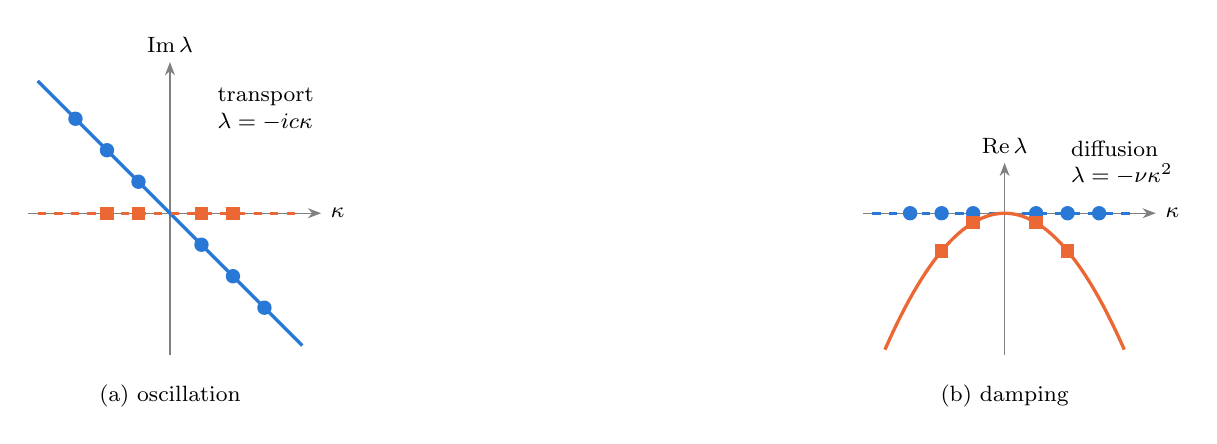
\begin{tikzpicture}[x=0.40cm,y=0.40cm,>=Stealth,font=\footnotesize]
  \begin{scope}
    \draw[->,gray] (-4.5,0)--(4.8,0) node[right,black]{$\kappa$};
    \draw[->,gray] (0,-4.5)--(0,4.8) node[above,black]{$\operatorname{Im}\lambda$};
    \draw[very thick,color={rgb,255:red,42;green,120;blue,214}] (-4.2,4.2)--(4.2,-4.2);
    \draw[very thick,color={rgb,255:red,235;green,104;blue,52},dashed] (-4.2,0)--(4.2,0);
    \foreach \k in {-3,-2,-1,1,2,3} \fill[color={rgb,255:red,42;green,120;blue,214}] (\k,-\k) circle (2.6pt);
    \foreach \k in {-2,-1,1,2} \fill[color={rgb,255:red,235;green,104;blue,52}] (\k,0) +(-2.4pt,-2.4pt) rectangle +(2.4pt,2.4pt);
    \node[anchor=west,align=left] at (1.2,3.3) {transport\\$\lambda=-ic\kappa$};
    \node at (0,-5.8) {(a) oscillation};
  \end{scope}
  \begin{scope}[xshift=10.6cm]
    \draw[->,gray] (-4.5,0)--(4.8,0) node[right,black]{$\kappa$};
    \draw[->,gray] (0,-4.5)--(0,1.6) node[above,black]{$\operatorname{Re}\lambda$};
    \draw[very thick,color={rgb,255:red,42;green,120;blue,214},dashed] (-4.2,0)--(4.2,0);
    \draw[very thick,color={rgb,255:red,235;green,104;blue,52},domain=-3.8:3.8,samples=60] plot (\x,{-0.3*\x*\x});
    \foreach \k in {-3,-2,-1,1,2,3} \fill[color={rgb,255:red,42;green,120;blue,214}] (\k,0) circle (2.6pt);
    \foreach \k in {-2,-1,1,2} \fill[color={rgb,255:red,235;green,104;blue,52}] (\k,{-0.3*\k*\k}) +(-2.4pt,-2.4pt) rectangle +(2.4pt,2.4pt);
    \node[anchor=west,align=left] at (1.8,1.6) {diffusion\\$\lambda=-\nu\kappa^2$};
    \node at (0,-5.8) {(b) damping};
  \end{scope}
\end{tikzpicture}
\caption{The idea of the paper on $(\partial_t+c\,\partial_x)(\partial_t-\nu\,\partial_x^2)u=0$. Every Fourier mode
$e^{\lambda t+i\kappa x}$ of a solution lies on the zero set of one factor of the symbol $(\tau+c\xi)(\tau-\nu\xi^2)$:
circles on the line of the transport factor, squares on the parabola of the diffusion factor (schematic;
\cref{fig:directions} shows the modes found in noisy data). Learning the equation means learning these two
groups.}\label{fig:branches}
\end{figure}

\paragraph{What the theory says} Three questions decide whether this clustering is well posed, and
\cref{sec:theory} answers each. \emph{Are the groups really the factors?} Yes: every solution splits into one
component per factor, uniquely up to an overlap whose dimension is the number of intersection points of the zero sets
(\cref{thm:factor}); additive terms, by contrast, admit no such split (\cref{prop:terms}). \emph{How well can the
groups be separated?} Exactly as well as the Friedrichs angle between the factors' solution spaces allows
(\cref{thm:hm}). \emph{What can finite data establish?} They can support a factored equation but never certify it
(\cref{prop:certify}); this is why the algorithm reports labels, not ``identified''.

\paragraph{What the algorithm does} It groups twice (\cref{fig:roadmap}). \emph{Within one sample} of the field it
reads the temporal rates of every wavenumber (the points of \cref{fig:branches}) and clusters them onto the curves of
candidate factors. \emph{Across posterior samples} it clusters the factors found in each sample, with a Dirichlet-process
mixture, so that the uncertainty of the data becomes a distribution over equations. Every decision is finally checked
against the raw observations, and the output carries intervals, the separation of each group and a label.

\begin{figure}[tbp]
\centering
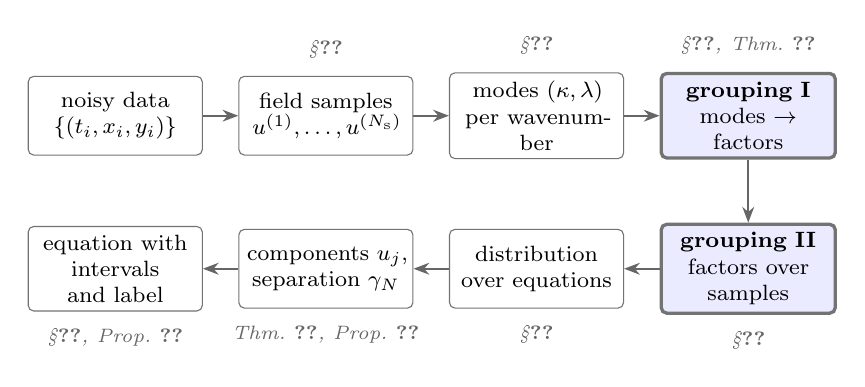
\begin{tikzpicture}[
  node distance=3.5mm and 4.5mm,
  box/.style={draw=black!55, rounded corners=2pt, align=center, font=\footnotesize, inner sep=3pt,
              minimum height=10mm, text width=20mm, fill=white},
  grp/.style={box, fill=blue!8, very thick},
  thy/.style={font=\scriptsize\itshape, text=black!60, align=center},
  arr/.style={-{Stealth[length=2mm]}, black!60, thick}]
\node[box] (data) {noisy data\\$\{(t_i,x_i,y_i)\}$};
\node[box, right=of data] (gp) {field samples\\$u^{(1)},\dots,u^{(\Nsamp)}$};
\node[box, right=of gp] (modes) {modes $(\kappa,\lambda)$\\per wavenumber};
\node[grp, right=of modes] (fac) {\textbf{grouping I}\\modes $\to$ factors};
\node[grp, below=8mm of fac] (cloud) {\textbf{grouping II}\\factors over samples};
\node[box, left=of cloud] (clus) {distribution\\over equations};
\node[box, left=of clus] (split) {components $u_j$,\\separation $\gN$};
\node[box, left=of split] (out) {equation with\\intervals and label};
\draw[arr] (data)--(gp); \draw[arr] (gp)--(modes); \draw[arr] (modes)--(fac);
\draw[arr] (fac)--(cloud); \draw[arr] (cloud)--(clus); \draw[arr] (clus)--(split); \draw[arr] (split)--(out);
\node[thy, above=1mm of gp] {\S\ref{sec:modes}};
\node[thy, above=1mm of modes] {\S\ref{sec:modes}};
\node[thy, above=1mm of fac] {\S\ref{sec:group1}, Thm.~\ref{thm:factor}};
\node[thy, below=1mm of cloud] {\S\ref{sec:group2}};
\node[thy, below=1mm of clus] {\S\ref{sec:group2}};
\node[thy, below=1mm of split] {Thm.~\ref{thm:hm}, Prop.~\ref{prop:bayes-angle}};
\node[thy, below=1mm of out] {\S\ref{sec:labels}, Prop.~\ref{prop:certify}};
\end{tikzpicture}
\caption{The method at a glance. The two grouping steps (thick boxes) are the core of the paper: modes are clustered
onto the curves of the factors within one sample, and factors are clustered across posterior samples. Each box names
the section that describes it and the result that justifies it.}\label{fig:roadmap}
\end{figure}

\paragraph{Contributions}
\begin{enumerate}
  \item \emph{The grouping principle and its limits}: groups are factors, with the exact ambiguity $\deltaP$
  (\cref{thm:factor}); terms are not groups (\cref{prop:terms}); the conditioning of the split (\cref{thm:hm}) and its
  Bayesian form (\cref{prop:bayes-angle}); what finite data can certify (\cref{thm:ident,prop:certify}).
  \item \emph{An algorithm that learns the groups} from noisy, gridded or scattered data, by clustering modes onto
  curves and factors across samples, whose output encodes these limits as intervals and labels.
  \item \emph{Evidence}: on $285$ random equations never used in development, $96.5\%$ right or equivalent and no
  confident wrong answer, against $28.4\%$ and $204$ confident wrong answers for weak SINDy; on a ten-equation
  benchmark in three designs, $30$ of $30$ factor sets.
\end{enumerate}

\paragraph{Relation to prior work}
Most methods that learn a PDE from data regress a time derivative on a library of candidate terms: SINDy and
PDE-FIND~\cite{BruProKut16,RudBruProKut17}, their weak, ensemble and Bayesian variants~\cite{MesBor21,FasKutBru22,HirBarKut22},
and Gaussian-process formulations of linear operators~\cite{RaiPerKar17}. Their unit is the \emph{term}. Dynamic mode
decomposition~\cite{Sch10,SasKut22} works with eigenvalues, as we do, but returns a linear operator on the data, not an
equation, and does not group eigenvalues by the factor they belong to. Matrix pencils~\cite{HuaSar90}, the algebra of
constant-coefficient operators and the Ehrenpreis--Palamodov fundamental principle~\cite{Ehr70,Pal70,Mal56,Hor90,Obe90},
and Dirichlet-process mixtures~\cite{BleJor06} are classical. What is new is the connection: the \emph{factor} of the
symbol, not the term, as the unit of learning; what finite data can certify about it and how stably it can be
separated; and an algorithm that groups twice and reports these limits.

\paragraph{Scope} Everything proved and implemented concerns scalar linear equations with constant coefficients in one
time and one space variable, observed on a rectangle. Equation~\eqref{eq:intro-tpd} with $c=1$, $\nu=0.3$ is the running
example. The proofs of the main results, the complete algorithm with its parameters, further cases, a guide to reading the
output, and the code and benchmark data are in the supplementary materials; the code is public~\cite{Pri26code}.

\section{The grouping principle}\label{sec:theory}
This section makes the picture of \cref{fig:branches} precise. Operators become polynomials (\cref{sec:ring}); the
factors of the polynomial split every solution, and terms do not (\cref{sec:factor}); the split is as stable as the angle
between the factors' solution spaces (\cref{sec:cond}); and finite data can support but not certify the result
(\cref{sec:certify}). Each subsection ends with the rule it gives to the algorithm. Proofs are in \SMproofs.

\subsection{Derivatives become polynomials}\label{sec:ring}
Every operator we consider has constant coefficients,
$P(\partial_t,\partial_x)=\sum_{j,k}c_{jk}\,\partial_t^j\partial_x^k$ with $c_{jk}\in\C$. The exponentials $\psi_{\tau,\xi}(t,x)=e^{\tau t+\xi x}$ are common eigenfunctions of all such operators:
\begin{equation}\label{eq:eigen}
  P(\partial)\,\psi_{\tau,\xi}=P(\tau,\xi)\,\psi_{\tau,\xi}.
\end{equation}
Differentiation becomes multiplication, and operators become polynomials.

\begin{definition}[Symbol and characteristic variety]\label{def:ring}
The constant-coefficient operators form the commutative ring $\ring=\C[\partial_t,\partial_x]\cong\C[\tau,\xi]$. The
polynomial $P(\tau,\xi)$ is the \emph{symbol} of $P(\partial)$, and its zero set
$\Var(P)=\{(\tau,\xi)\in\C^2:P(\tau,\xi)=0\}$ is the \emph{characteristic variety}.
\end{definition}

By \eqref{eq:eigen}, $\psi_{\tau,\xi}$ solves $P(\partial)u=0$ exactly when $(\tau,\xi)\in\Var(P)$. A Fourier mode in
space is the case $\xi=i\kappa$ with wavenumber $\kappa\in\R$; then $P(\lambda,i\kappa)=0$ is the \emph{dispersion
relation}, and its roots $\lambda(\kappa)$ are the \emph{temporal rates} of the modes $e^{\lambda(\kappa)t+i\kappa x}$.
The real part of a rate is growth or decay, the imaginary part is oscillation. We keep $\xi$ in statements about the
ring and set $\xi=i\kappa$ only on Fourier modes, so that a real equation has a symbol with real coefficients.

\begin{example}[Running example]\label{ex:running}
$P=(\partial_t+c\,\partial_x)(\partial_t-\nu\,\partial_x^2)$ has symbol $P=Q_1Q_2$ with $Q_1=\tau+c\,\xi$ and
$Q_2=\tau-\nu\,\xi^2$. On Fourier modes the two factors give two branches of rates, $\lambda_1(\kappa)=-ic\kappa$ (a
wave that travels without decay) and $\lambda_2(\kappa)=-\nu\kappa^2$ (a standing mode that decays). A solution is any
superposition of modes on the two branches. The equation is one object; its two factors are two groups of modes.
\end{example}

\subsection{Groups are factors, not terms}\label{sec:factor}
Let the symbol be factored into pairwise coprime factors,
\begin{equation}\label{eq:factored}
  P=Q_1\cdots Q_N,\qquad Q_j=P_j^{e_j},
\end{equation}
with $P_j$ irreducible and $e_j$ its multiplicity. Two ways of splitting a solution suggest themselves: one piece per
factor $Q_j$, or one piece per additive term of the operator (for $u_t=\nu u_{xx}-cu_x$, one piece for diffusion and one
for transport). Only the first works.

\begin{theorem}[Factor decomposition]\label{thm:factor}
Let $\Omega\subset\R^2$ be bounded, connected and simply connected, and let $P$ be as in \eqref{eq:factored}. Every
solution $u$ of $P(\partial)u=0$ on $\Omega$ (a distribution or a smooth function) can be written
\begin{equation}\label{eq:split}
  u=\sum_{j=1}^Nu_j,\qquad Q_j(\partial)\,u_j=0 .
\end{equation}
The tuples $(u_1,\dots,u_N)$ that sum to zero form a space of exponential-polynomials of dimension exactly
\begin{equation}\label{eq:delta}
  \deltaP=\sum_{i<j}\dim_\C\ring/(Q_i,Q_j),
\end{equation}
the number of intersection points of the varieties $\Var(Q_i)$, counted pair by pair and with multiplicity.
\end{theorem}

The theorem says that the decomposition \emph{exists} and that its only freedom has finite dimension. Each meeting point
of two curves $\Var(Q_i)$ and $\Var(Q_j)$ is a mode that solves both factors and can therefore be moved from one group to
the other without changing $u$. In one variable the statement is B\'ezout's identity: from $aQ_1+bQ_2=1$
follows the split $u=bQ_2u+aQ_1u$. In two variables coprime factors no longer generate $1$; they only have finitely many common
zeros, and $\deltaP$ counts exactly that defect. The hypotheses matter: on a domain with a hole the Laplacian factors as
$(\partial_x+i\partial_y)(\partial_x-i\partial_y)$, yet its solution $\log\abs{z}^2$ on an annulus is not a sum of a
holomorphic and an antiholomorphic single-valued function. This is why the algorithm works on rectangles.

\begin{example}[Running example: two groups, two shared modes]\label{ex:delta}
$Q_1=\tau+c\xi$ and $Q_2=\tau-\nu\xi^2$ meet at $(0,0)$ and $(c^2/\nu,-c/\nu)$, so $\deltaP=2$: a constant and the
exponential $e^{(c^2/\nu)t-(c/\nu)x}$ can be moved between the groups. Among Fourier modes only the first is visible:
the $\kappa=0$ mode belongs to both groups.
\end{example}

\paragraph{The groups are read from the rates} When every factor is an evolution factor, $Q_j=\tau-\Lambda_j(\xi)$, the
component $u_j$ is obtained from $u$ by a Fourier multiplier. On a wavenumber $\kappa$ at which no two branches meet,
\begin{equation}\label{eq:lagrange}
  \hat u_j(t,\kappa)=\prod_{k\neq j}\frac{\partial_t-\Lambda_k(i\kappa)}{\Lambda_j(i\kappa)-\Lambda_k(i\kappa)}\;\hat u(t,\kappa),
\end{equation}
the Lagrange formula for the spectral projectors of $\partial_t$ restricted to that wavenumber. \emph{The rates decide
the groups}, and the poles of the multiplier sit exactly at the visible part of the overlap $\deltaP$. This is what the
algorithm exploits: it never needs the operator in advance, only the rates and their arrangement on curves.

\paragraph{Why additive terms do not form groups}
\begin{proposition}[Terms do not give components]\label{prop:terms}
If $P=A_1+A_2$ with constant coefficients, then every solution of $P(\partial)u=0$ that is a sum $a+b$ with $A_1a=0$
and $A_2b=0$ also solves $A_1A_2u=0$. If $\Var(A_1)\cap\Var(A_2)$ is finite, these solutions form a finite-dimensional
space of exponential-polynomials.
\end{proposition}
\begin{proof}[Proof sketch]
$A_1A_2(a+b)=A_2A_1a+A_1A_2b=0$ because the operators commute. A common zero of $P$ and $A_1A_2$ is a common zero of $A_1$
and $A_2$, so the joint kernel of $P$ and $A_1A_2$ lives on a finite set of exponents.
\end{proof}

For the heat equation, $A_1=\partial_t$ and $A_2=-\nu\partial_x^2$: a ``stationary part plus a diffusion part''
$f(x)+a(t)+b(t)x$ is killed by $\partial_t\partial_x^2$, while a single heat mode $e^{-\nu\kappa^2t}\cos\kappa x$ is not. A
generic solution is not a sum of single-term pieces. What a term-wise split leaves over is the \emph{interaction} of the
terms; it is as large as the solution itself, and on a non-periodic window it cannot be removed by any continuous,
hence any regularized, procedure (\SMinteraction). Different factors, in contrast, superpose exactly: \emph{factors, not
terms, are the groups.}

\roleinalg{The objects to cluster are modes, and a cluster is a factor: a curve $\Var(Q_j)$ in the plane of rates. The
overlap $\deltaP$ is the irreducible ambiguity; the algorithm resolves it by a fixed convention (\cref{sec:group1}).
Because the interaction of terms cannot be regularized away, the algorithm uses no coefficient penalty.}

\subsection{How well separated are the groups? The Friedrichs angle}\label{sec:cond}
\Cref{thm:factor} says that the split exists, not that it is stable. Let $M_j=\ker_{\Hs}Q_j$ be the solutions of factor
$j$ in the Sobolev space $\Hs(\Omega)$, let $\sumop(u_1,\dots,u_N)=\sum_ju_j$ be the sum operator, and define its
conditioning constant
\begin{equation}\label{eq:gammaN}
  \gN=\inf_{0\neq v\perp\ker\sumop}\frac{\norm{\sumop v}^2}{\norm{v}^2},\qquad \norm{(u_1,\dots,u_N)}^2=\sum_j\norm{u_j}_{\Hs}^2 .
\end{equation}
It is the worst case, over all tuples of pieces, of the size of the sum relative to the size of the pieces. If the
spaces are orthogonal, $\gN=1$; if $M_2$ approaches $M_1$, one can take $u_2\approx-u_1$, the pieces stay of unit size
while their sum vanishes, and $\gN\to0$. For two groups $\gamma_2=1-\cF$, where $\cF=\cos\thetaF$ is the cosine of the
smallest nonzero angle between $M_1$ and $M_2$, the \emph{Friedrichs angle}~\cite{Deu01} (\cref{fig:friedrichs}). In
regression terms $M_1$ and $M_2$ are two blocks of regressors, and $\cF$ is the largest correlation between a combination
of the first block and one of the second.

\begin{figure}[tbp]
\centering
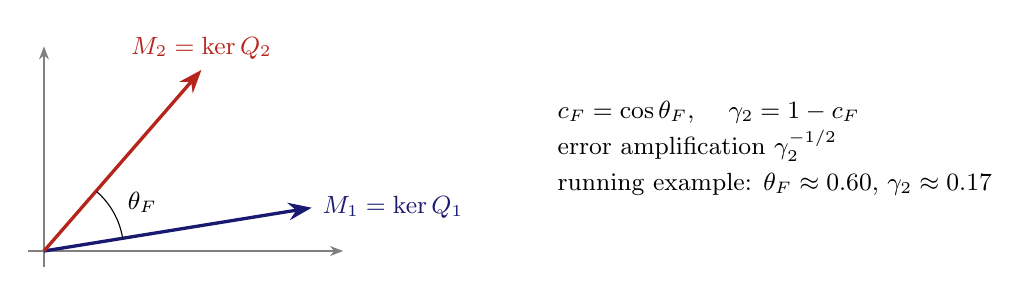
\begin{tikzpicture}[scale=1.0,>=Stealth]
  \draw[->,gray] (-0.2,0)--(3.8,0); \draw[->,gray] (0,-0.2)--(0,2.6);
  \draw[very thick,->,color=MidnightBlue] (0,0)--(3.4,0.55) node[right]{\small $M_1=\ker Q_1$};
  \draw[very thick,->,color=BrickRed] (0,0)--(2.0,2.3) node[above]{\small $M_2=\ker Q_2$};
  \draw (1.0,0.16) arc (9.2:49:1.0); \node at (1.25,0.62) {\small$\thetaF$};
  \node[anchor=west,align=left,font=\small] at (6.4,1.3)
   {$\cF=\cos\thetaF$, \quad $\gamma_2=1-\cF$\\[2pt]
    error amplification $\gamma_2^{-1/2}$\\[2pt]
    running example: $\thetaF\approx0.60$, $\gamma_2\approx0.17$};
\end{tikzpicture}
\caption{The Friedrichs angle between the solution spaces of two factors. A small angle means that large pieces can
almost cancel, so recovering the pieces from their sum amplifies errors by up to $\gamma_2^{-1/2}=(1-\cos\thetaF)^{-1/2}$.
The values are those measured on the running example (\cref{sec:worked}).}\label{fig:friedrichs}
\end{figure}

\begin{theorem}[Stability of the split]\label{thm:hm}
Every $u\in\ker_{\Hs}P$ has components $u_j\in\Hs$ if and only if $\sum_jM_j$ is closed and dense in $\ker_{\Hs}P$.
Closedness is equivalent to $\gN>0$, and then the minimum-norm components satisfy
\begin{equation}\label{eq:hm}
  \Big(\sum_j\norm{u_j}_{\Hs}^2\Big)^{1/2}\le\gN^{-1/2}\,\norm{u}_{\Hs}.
\end{equation}
For the finite-dimensional sampled kernels used by the algorithm the sum is always closed, and stability reduces to
$\gN>0$.
\end{theorem}

Two remarks keep the theorem honest. On infinite-dimensional component spaces $\gN>0$ can fail, and the pieces of a
smooth $u$ may be one derivative rougher than $u$. For $N\ge3$ groups the pairwise angles do not determine $\gN$: three
spaces can be pairwise well separated and jointly nearly dependent, so the full Gram operator of $\sumop$ is needed.

\roleinalg{$\gN$ is computed on the sampled kernels and reported with every result. It sets the width of the intervals of
the components (\cref{prop:bayes-angle}): closely aligned groups are never hidden; they show up as wide intervals,
not as a confident but wrong split.}

\subsection{What finite data can and cannot certify}\label{sec:certify}
When does a solution determine its equation? Let the \emph{annihilator} $\Ann(u)=\{Q\in\ring:Q(\partial)u=0\}$ collect
every constant-coefficient equation that $u$ satisfies; it is an ideal of $\ring$. The question is whether
$\Ann(u)=(P)$, i.e.\ whether every equation $u$ satisfies is a consequence of $P$. The answer turns on one class of
functions.

\begin{definition}[Exponential-polynomials]\label{def:ep}
$\EP$ is the set of finite sums $\sum_jp_j(t,x)\,e^{\tau_jt+\xi_jx}$ with polynomials $p_j$ and exponents
$(\tau_j,\xi_j)\in\C^2$. Equivalently (\SMproofs), $w\in\EP$ if and only if the derivatives of $w$ span a
finite-dimensional space.
\end{definition}

An exponential-polynomial \emph{remembers too little}: it sits on finitely many points of $\C^2$, and through finitely
many points pass infinitely many curves, so infinitely many equations. A single heat mode $e^{-\nu\kappa^2t+i\kappa x}$
solves the heat equation, but equally the pure decay $\partial_t+\nu\kappa^2$ and every other equation whose variety
passes through $(-\nu\kappa^2,i\kappa)$. The heat kernel $t^{-1/2}e^{-x^2/(4\nu t)}$, whose derivatives span an
infinite-dimensional space, fills the whole curve, and every equation it satisfies is a multiple of $\partial_t-\nu\partial_x^2$.
The general statement strips one irreducible factor at a time.

\begin{theorem}[Identification]\label{thm:ident}
Let $\Omega$ be open and connected, $P(\partial)u=0$, and $P=\prod_iP_i^{e_i}$ with distinct irreducible $P_i$. Then
$\Ann(u)=(P)$ if and only if $(P/P_i)(\partial)u\notin\EP(\Omega)$ for every $i$. In that case $P$ is the unique
annihilator of minimal degree, up to a constant.
\end{theorem}

In words: $u$ determines its equation exactly when, after removing any one factor, what remains is still a genuine
solution of that factor, not a finite sum of modes. Data, however, are finitely many numbers, and finitely many numbers
are always matched by an exponential-polynomial.

\begin{proposition}[Finite data]\label{prop:certify}
Let $\Omega$ be connected and $z_0\in\Omega$. (i) If the derivatives of $u$ span a space of dimension at most $n$, the
derivatives of order at most $2n-1$ at $z_0$ determine $\Ann(u)$. (ii) Without such a bound, for every finite set of
derivatives at a point, and for every finite set of samples, there is an exponential-polynomial that matches them; hence
no finite data prove $\Ann(u)=(P)$.
\end{proposition}

\roleinalg{An algorithm can refute a candidate equation, or report that it is compatible with the data at the available
resolution, but it can never certify it. The output therefore carries a label (\cref{sec:labels}), and the label that
plays the role of ``identified'' requires each factor to be seen at enough distinct wavenumbers to pin it down within
its class (\cref{prop:counting}).}

\section{Learning the groups}\label{sec:algorithm}
The algorithm turns the data into modes (\cref{sec:modes}), clusters the modes onto the curves of factors within each
sample of the field (grouping I, \cref{sec:group1}) inside a class of operators chosen by the data
(\cref{sec:class}), clusters the factors across samples (grouping II, \cref{sec:group2}), and labels the result
(\cref{sec:labels}). The complete algorithm, with every parameter and its default, is in \SMalgo.

\subsection{From data to modes}\label{sec:modes}
\paragraph{Field samples} The input is a set of noisy observations $y_i=u(t_i,x_i)+\varepsilon_i$,
$\varepsilon_i\sim\Normal(0,\noise^2)$, on a window $[0,T]\times[0,L)$ periodic in $x$, or a noisy field on a regular grid.
Scattered observations are interpolated by a Gaussian process whose kernel is a sum of separable Mat\'ern-$5/2$
products (a transported profile and a diffusing one do not share a length scale), with the hyperparameters integrated
out by importance sampling. The output of this stage is not the posterior mean but $\Nsamp$ posterior \emph{samples}
$u^{(q)}$ of the field, each with a weight $\pi_q$. The reason is structural: the maps applied next are not continuous
(factors of a numerical symbol jump where it becomes reducible), so the mean of the outputs differs from the output of
the mean, and the mean, a Wiener filter, shrinks exactly the fast-decaying high-wavenumber modes that carry the
diffusive factors. On gridded input the noisy grid itself is used, and parametric-bootstrap refits provide the spread.

\paragraph{The usable band} Not every wavenumber carries information about the symbol. Three limits apply: spatial
aliasing ($\abs{\kappa}\le\pi/\Delta x$); temporal aliasing along a branch, since a rate is read from samples spaced by
$\Delta t$ only modulo $2\pi i/\Delta t$; and, usually the binding one, noise together with decay. After the spatial Fourier
transform one wavenumber bin carries noise of standard deviation $\sigbin=\noise/\sqrt{n_x}$, and a mode is used only
while its amplitude exceeds $z\,\sigbin$ ($z=3$). A diffusive mode of rate $-\nu\kappa^2$ falls below this threshold after
a time of order
\[
  t_\kappa\approx\frac{\log\big(\abs{A_\kappa}/z\sigbin\big)}{\nu\kappa^2},
\]
so the high wavenumbers of a dissipative group are lost
first. This is a property of the data, not of the method. The band $\mathcal K$ is the set of wavenumbers that pass all
three limits. It must hold enough distinct wavenumbers per group:

\begin{proposition}[Counting condition]\label{prop:counting}
Let $Q=\tau-\Lambda(\xi)$ with $\Lambda$ a polynomial of degree at most $d$. Its coefficients are determined by the rates
$\lambda(\kappa_\ell)=\Lambda(i\kappa_\ell)$ at $d+1$ distinct wavenumbers, and not by fewer; the coefficient error is at
most $\norm{V^{-1}}\max_\ell\abs{\delta\lambda_\ell}$ with $V=((i\kappa_\ell)^k)$ the Vandermonde matrix, whose inverse grows
like $h_\kappa^{-d}$ when the nodes cluster within a spread $h_\kappa$~\cite{Gau62}. For real coefficients
$\lfloor d/2\rfloor+1$ distinct values of $\abs{\kappa}$ suffice.
\end{proposition}

So the whole band is used, not the cleanest few bins: spreading the wavenumbers is what keeps $V$ well conditioned.

\paragraph{Rates by the matrix pencil} For each sample and each $\kappa\in\mathcal K$, the spatial Fourier transform gives
a time series that, for a constant-coefficient equation, is a sum of exponentials, one per root of the symbol at that
wavenumber:
\begin{equation}\label{eq:expsum}
  \hat u(t,\kappa)=\sum_{p=1}^{r(\kappa)}A_p\,e^{\lambda_p(\kappa)t},\qquad Q_{j(p)}\big(\lambda_p,i\kappa\big)=0 .
\end{equation}
The rates are the eigenvalues of $\partial_t$ on the space spanned by the series and its shifts, and the matrix pencil
method computes them~\cite{HuaSar90}. From the Hankel matrix $H_{\ell k}=\hat u(t_{\ell+k},\kappa)$ take $Y_0$ ($H$ without
its last column) and $Y_1$ ($H$ without its first), both projected on the $r$ leading singular directions. Advancing a
series by one step multiplies the term $A_pe^{\lambda_pt}$ by $\mu_p=e^{\lambda_p\Delta t}$, so
\begin{equation}\label{eq:pencil}
  \lambda_p=\tfrac{1}{\Delta t}\log\mu_p,\qquad \mu_p\in\operatorname{eig}\big(Y_0^{+}Y_1\big).
\end{equation}
The order $r$ is chosen per bin by BIC, and each rate receives a standard deviation $\sigma_{\lambda,p}$ from the
Cram\'er--Rao bound of model \eqref{eq:expsum}; weak, fast-decaying or nearly coincident modes receive large ones.
This step does \emph{not} fit the equation: it returns a cloud of points $(\kappa,\lambda_p(\kappa))$ with error bars, the
noisy version of \cref{fig:branches}. Two rates closer than about $4/T$ cannot be resolved in a window of length $T$; such
bins are flagged as confluent.

\subsection{Grouping I: modes onto curves}\label{sec:group1}
The obvious route, fitting one polynomial through all points and factoring it, is ill-posed: a polynomial with noisy
coefficients is almost never reducible, and when it is, its factors move discontinuously with the coefficients (in our
tests this route split the irreducible Klein--Gordon and telegraph symbols at noise $10^{-4}$). We therefore group and fit
at the same time. Given a structure $\Mfit$ (the number $N$ of factors and their degrees, \cref{sec:class}), we solve the
\emph{$N$-varieties problem}, a version of $k$-means in which the cluster centres are curves instead of points: assign
every mode to the factor whose variety is nearest, refit each factor to the modes assigned to it, and repeat until the
assignment stops changing. The distance of mode $p$ to factor $Q_j$ is its first-order distance to the variety in units
of its own uncertainty,
\begin{equation}\label{eq:dist}
  r_j(p)=\frac{\abs{Q_j(\lambda_p,i\kappa_p)}}{\sigma_{\lambda,p}\,\abs{\partial_\tau Q_j(\lambda_p,i\kappa_p)}},
\end{equation}
and each mode costs $\min(r_j(p)^2,9)$, so an isolated outlier pays a fixed penalty instead of dragging a curve away.
This is the grouping of \cref{thm:factor} learned directly from the spectrum.

\begin{figure}[tbp]
\centering
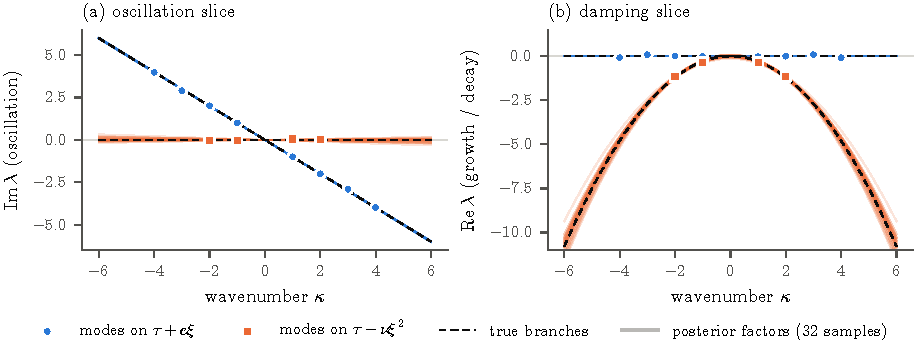
\includegraphics[width=\linewidth]{fig_directions}
\caption{Grouping I on the running example ($64\times128$ grid, $5\%$ noise). Points: modes found by the matrix pencil,
coloured by the factor they were assigned to. Dashed: the true branches $\lambda=-ic\kappa$ and $\lambda=-\nu\kappa^2$.
Thin lines: the factors fitted to $32$ posterior samples; they bundle where there are modes and fan out where there are
none. (a) Oscillation $\operatorname{Im}\lambda$: transport is the sloped line, diffusion the flat one. (b) Damping
$\operatorname{Re}\lambda$: transport is flat at zero, diffusion the downward parabola.}\label{fig:directions}
\end{figure}

\Cref{fig:directions} shows the result on the running example. Each factor is a direction in the plane of rates, and the
modes of one group line up along it. Once modes are assigned, the component of group $j$ is the sum of its modes,
\begin{equation}\label{eq:components}
  u_j(t,x)=\sum_{p:\,j(p)=j}A_p\,e^{\lambda_p(t-t_0)+i\kappa_px},
\end{equation}
the discrete counterpart of the projector \eqref{eq:lagrange}. A
mode within distance $3$ of two varieties lies in the overlap $\deltaP$ (for the running example, $\kappa=0$) and is split
equally between the groups: among all splits allowed by \cref{thm:factor} this one puts the least energy into the
ambiguity, and it coincides with the posterior mean of \cref{prop:bayes-angle}. The energy shares
$w_j=\norm{u_j}/\sum_k\norm{u_k}$ follow. A group can itself split further (two conjugate branches of the beam equation are
first found as one factor of degree two in $\tau$); each component is therefore analysed again, and a split is kept only
if it leaves the kernel unchanged or improves the evidence of \cref{sec:labels}.

\subsection{Choosing the class of operators}\label{sec:class}
A structure $\Mfit=((m_1,d_1),\dots,(m_N,d_N))$ fixes $N$ and, for each factor, its degree $m_j$ in $\tau$ and $d_j$ in
$\xi$; the running example is $((1,1),(1,2))$. The class $C(m,d)$ holds all structures with $\sum_jm_j\le m$ and
$d_j\le d$. Grouping I is run for every structure, and structures are compared by
\begin{align}
  \mathrm{BIC}(\Mfit)&=2n_m\log\max\!\Big(\frac{\chi^2}{2n_m},\,1\Big)+n_{\mathrm{par}}(\Mfit)\log(2n_m),\label{eq:bic}\\
  P(\Mfit\mid\text{data})&\propto e^{-\mathrm{BIC}(\Mfit)/2},\label{eq:pstruct}
\end{align}
where $\chi^2$ is the total capped misfit of the $n_m$ modes and $n_{\mathrm{par}}$ the number of coefficients. The floor
$\max(\cdot,1)$ means that misfit is penalized only once it exceeds what the noise explains, so a fit better than the
noise is never rewarded. The class is grown from $C(3,4)$ (90 structures) up to $C(4,8)$ (1353) only when the data demand
it, i.e.\ when most of the posterior mass is on structures that fail the tests of \cref{sec:labels}, and a larger class is
kept only if it also predicts the second half of the time window from the first. This is the only regularization of the
method, and it acts on the class, by Occam's razor, not on the coefficients: by \cref{sec:factor} a coefficient penalty
cannot remove the interaction of terms, and by \cref{thm:hm} it can push the error of the split below its floor only by
shrinking the components, which the next layer does explicitly and reports.

\subsection{Grouping II: factors across samples}\label{sec:group2}
Grouping I gives one set of factors per field sample. Two questions remain: how well are the components determined given
the factors, and which factors of different samples are the same factor?

\paragraph{The angle sets the error bars} On the observation window write $u=\sum_jB_ja_j+\varepsilon=\sumop a+\varepsilon$,
with $B_j$ an orthonormal basis of the sampled kernel of $Q_j$, $\varepsilon\sim\Normal(0,\noise^2I)$ and a Gaussian prior
$a\sim\Normal(0,\omega^2I)$, whose scale $\omega^2$ is set by empirical Bayes. The posterior of the coefficients is Gaussian,
\begin{equation}\label{eq:posterior-a}
  a\mid u\sim\Normal(\hat a,\Gamma_a),\qquad
  \Gamma_a=\noise^2\Big(\sumop^H\sumop+\frac{\noise^2}{\omega^2}\,I\Big)^{-1};
\end{equation}
the layer returns a distribution of splits, not one split.

\begin{proposition}[The angle sets the error bars]\label{prop:bayes-angle}
For two groups the eigenvalues of $\sumop^H\sumop$ are $1\pm\cos\theta_k$, with $\theta_k$ the principal angles between the
sampled kernels (and $1$ on the directions of the larger kernel without a partner). In the worst direction orthogonal to
$\ker\sumop$ the posterior variance of the component coefficients is
\begin{equation}\label{eq:bayes-angle}
  \frac{\noise^2}{\gamma_2+\noise^2/\omega^2},\qquad \gamma_2=1-\cF .
\end{equation}
On the shared directions ($\theta_k=0$, the overlap $\deltaP$) the posterior equals the prior, and its mean splits the
shared part equally.
\end{proposition}

This is the Bayesian form of \eqref{eq:hm}: intervals grow like $\noise/\sin(\thetaF/2)$ as the angle closes and are capped
by the prior when $\thetaF\to0$. The same evidence compares the two-factor model with the one-factor model and gives the
probability $P(\text{split})$, which returns to its prior as $\thetaF\to0$.

\paragraph{The cloud of factors} Each factor of each sample is mapped to the vector $\beta$ of its monic coefficients,
zero-padded to the largest degrees in play, and receives the mass of its sample times its energy share:
\begin{equation}\label{eq:cloud}
  \cloud=\sum_{q=1}^{\Nsamp}\pi_q\sum_jw_j^{(q)}\,\delta_{\beta_j^{(q)}} .
\end{equation}
A sharp equation is a cloud with a few tight clusters, an uncertain one a diffuse cloud. Since the number of groups is
unknown, the cloud is modelled by a Dirichlet-process Gaussian mixture~\cite{BleJor06} (truncated stick-breaking,
variational inference), which lets the data choose the number of clusters; two clusters that never occur in the same
sample are merged when one Gaussian explains them better. The cluster centres are the factors, quantiles over samples
give their $90\%$ intervals, and the cluster responsibilities give the posterior $P(k)$ of the number $k$ of groups.
\Cref{fig:grouping} shows the cloud of the running example.

\begin{figure}[tbp]
\centering
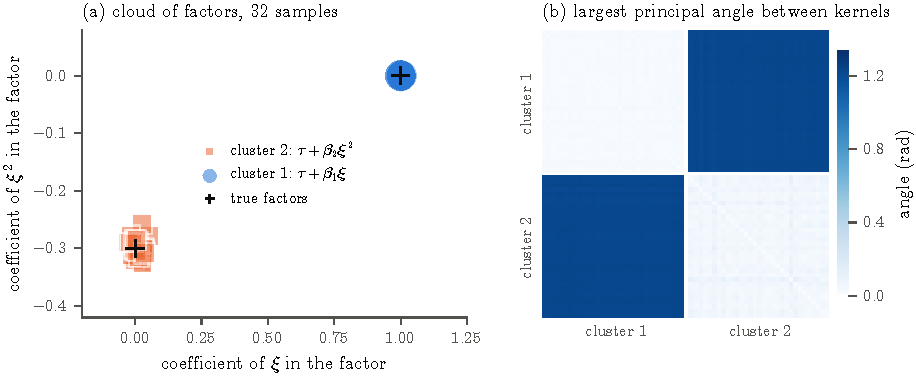
\includegraphics[width=\linewidth]{fig_grouping}
\caption{Grouping II on the running example. (a) Each marker is one factor found in one of $32$ posterior samples,
placed by its coefficients of $\xi$ and $\xi^2$; area is proportional to its mass $\pi_qw_j$; crosses mark the true
factors. The cloud has two tight clusters and nothing in between. (b) Largest principal angle between the sampled
kernels of every pair of factors, ordered by cluster: factors of the same group allow the same functions (light
diagonal blocks), factors of different groups do not (dark off-diagonal blocks).}\label{fig:grouping}
\end{figure}

\subsection{Decision and labels}\label{sec:labels}
The interpolated field has already smoothed the high wavenumbers, so the final decisions are made on the \emph{raw
observations}. A candidate set of factors defines a linear model $y=Ea+\varepsilon$ for the $n$ observations, where the
columns of $E$ are the kernel exponentials of the factors evaluated at the observation points. Integrating the
amplitudes out gives
\[
  y\mid Q_1,\dots,Q_N\sim\Normal\big(0,\ \noise^2I+\omega^2EE^H\big),
\]
and the score
\begin{equation}\label{eq:evidence}
  S(Q_1,\dots,Q_N)=\log\Normal\big(y;0,\noise^2I+\omega^2EE^H\big)-\tfrac12n_{\mathrm{par}}\log n
\end{equation}
decides between dropping a factor, dropping a term whose interval contains zero, merging two factors or splitting one;
a change needs more than one nat. The same model gives a goodness-of-fit statistic
\[
  \chi^2=\sum_{i=1}^n\frac{\abs{y_i-\hat y_i}^2}{\noise^2},
\]
with $\hat y$ the projection of $y$ on the columns of $E$, approximately chi-squared with $n-\rank E$ degrees of freedom. The result then receives one of four labels, which encode
what \cref{sec:certify} allows:

\smallskip
\noindent\begin{tabularx}{\linewidth}{@{}l X@{}}
\toprule
\FC & every factor has more modes than coefficients, at least $d_j+1$ distinct wavenumbers (\cref{prop:counting}), and
the fit passes the goodness-of-fit test: the data are compatible with the factored equation and pin it down within the class.\\
\IDK & the fit is good, but some factor is pinned down only relative to the declared class.\\
\MIS & the goodness-of-fit test rejects the structure ($p<10^{-3}$).\\
\UND & the data cannot decide, typically because of confluent rates or a repeated factor $P_i^2$, whose polynomial
prefactors $t\,e^{\lambda t}$ finite noisy data cannot separate from two nearby rates.\\
\bottomrule
\end{tabularx}
\smallskip

\noindent The output is therefore a distribution, never a point estimate: the factors with $90\%$ intervals, $P(k)$ and
the posterior over structures, the energy shares $w_j$ with intervals, $P(\text{split})$, the separation $\gN$, and the
label. A small Friedrichs angle does not reject the equation; it widens the intervals, so the reader always sees how well
each group is separated, not only whether the equation fits.

\section{Evidence}\label{sec:evidence}
We first follow one data set through both groupings (\cref{sec:worked}), then report the large benchmark on random
equations and the development benchmark (\cref{sec:bench}). An answer is \emph{right} if the recovered set of factors
matches the true one within relative coefficient error $0.05$; \emph{equivalent} if it explains the data as well as the
true equation (a $\chi^2$ test adjusted for degrees of freedom, or the same product written differently); an
\emph{abstention} if the label is \IDK{} or \UND; and \emph{false-confident} if a wrong equation is returned as if it
were right. Library-regression baselines cannot abstain, so each of their wrong answers is false-confident.

\subsection{One run, step by step}\label{sec:worked}
The data are the running example with $c=1$, $\nu=0.3$ on a $64\times128$ grid over $[0,2]\times[0,2\pi)$, with white
noise of standard deviation $0.05\,\mathrm{std}\abs{u}$. \emph{Modes}: only $\kappa\le4$ rise above the detection
threshold; the matrix pencil returns twelve modes. \emph{Grouping I} (\cref{fig:directions}): eight modes lie on the line
$\operatorname{Im}\lambda=-\kappa$ with $\operatorname{Re}\lambda\approx0$, four on the parabola $\operatorname{Re}\lambda=-0.3\kappa^2$;
the transport modes occupy eight distinct wavenumbers and the diffusion modes four, against two and three required by
\cref{prop:counting}. \emph{Class}: the structure $((1,1),(1,2))$ ranks first. \emph{Grouping II}
(\cref{fig:grouping}): over $32$ posterior samples the $64$ factors form two tight clusters, with masses $0.767$ and
$0.233$ and $P(k=2)=1$. \emph{Components} (\cref{fig:components}): the transport component consists of tilted stripes, a
profile moving at speed $1$; the diffusion component has vertical structure fading in time; the residual, $2.5\%$ of the
data norm, shows no structure. \Cref{tab:worked} lists the output. The groups are only moderately separated
($\thetaF=0.60$, amplification $\gN^{-1/2}=2.41$), and the intervals still cover the truth; the two conjugate factors of
the beam equation, much closer to each other ($\cF=0.939$), are recovered with the same accuracy and an amplification of
$4.05$ (\SMcases).

\begin{figure}[tbp]
\centering
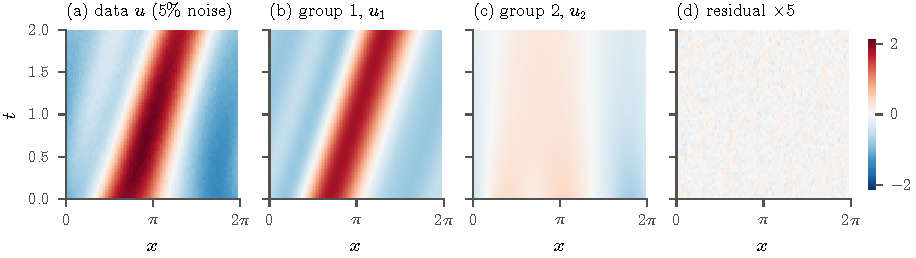
\includegraphics[width=\linewidth]{fig_components}
\caption{The worked example as functions of $(t,x)$ on a common colour scale: (a) noisy data; (b) transport component;
(c) diffusion component; (d) residual, magnified five times, indistinguishable from the noise.}\label{fig:components}
\end{figure}

\begin{table}[tbp]
\centering\small
\caption{Output of the worked example and how to read it. Intervals are $90\%$ intervals from $16$ parametric-bootstrap
refits.}\label{tab:worked}
\begin{tabularx}{\linewidth}{@{}l l X@{}}
\toprule
Quantity & Value & Meaning\\
\midrule
equation & $(\tau+1.0006\,\xi)(\tau-0.2980\,\xi^2)$ & recovered factors; truth $(\tau+\xi)(\tau-0.3\,\xi^2)$\\
coefficient of $\xi$ & $1.0006\ [0.9998,1.0020]$ & speed $c$ of the transport group\\
coefficient of $\xi^2$ & $-0.2980\ [-0.3049,-0.2919]$ & diffusivity $\nu$ of the diffusion group\\
label & \FC & enough distinct wavenumbers per factor; goodness of fit passed\\
$P(k)$; $P(\text{split})$ & $P(k=2)=1$; $1.000$ & number of groups; evidence that both groups are needed\\
$w_1,\ w_2$ & $0.768,\ 0.232$ & energy shares of the two groups\\
$\gN,\ \thetaF$; $\gN^{-1/2}$ & $0.173,\ 0.60$; $2.41$ & separation of the groups; worst-case error amplification\\
\bottomrule
\end{tabularx}
\end{table}

\subsection{Benchmarks}\label{sec:bench}
\paragraph{Large benchmark on random equations} To test generalization we drew $300$ equations at random from five
families, $60$ each: first-order factors (F1); first-order dispersive factors (F2); irreducible
second-order factors (F3); products of two or three factors (F4); and third-order factors or a reaction factor times a
transport factor, often with few excited wavenumbers (F5). Every draw is a different equation with an independent field
and independent noise ($1\%$ of $\mathrm{std}\abs{u}$, regular grid), and none was used to set any parameter: the pipeline
ran with the defaults fixed during development. We compare with weak SINDy~\cite{MesBor21}, the strongest library
regression on the development benchmark below, run through PySINDy with a linear library of mixed derivatives and a
sparsity threshold chosen by BIC. $285$ draws finished; $15$ (twelve in F4, three in F5) exceeded the time limit of three
hours per draw and are reported separately. \Cref{tab:large} and \cref{fig:evidence}(a) give the outcomes.

\begin{table}[tbp]
\centering\small
\caption{Large benchmark: $285$ random equations not used in development, grid, $1\%$ noise. ``Right+eq.'' is the share
of right or equivalent answers with a Wilson $95\%$ interval; ``abstain'' includes one correct abstention (F2) and one
crash (F4).}\label{tab:large}
\begin{tabular}{@{}llrrrrr@{\hspace{14pt}}l@{}}
\toprule
family & method & $n$ & right & equiv. & abstain & false-conf. & right+eq.\\
\midrule
all & this method & 285 & 187 & 88 & 10 & \textbf{0} & \textbf{96.5\%} [93.7, 98.1]\\
    & weak SINDy  & 285 &  77 &  4 &  0 & 204 & 28.4\% [23.5, 33.9]\\
\midrule
F1 & this method & 60 & 59 &  1 & 0 & 0 & 100\%\\
   & weak SINDy  & 60 & 42 &  0 & 0 & 18 & 70.0\%\\
F2 & this method & 60 & 31 & 23 & 6 & 0 & 90.0\%\\
   & weak SINDy  & 60 &  9 &  0 & 0 & 51 & 15.0\%\\
F3 & this method & 60 & 41 & 18 & 1 & 0 & 98.3\%\\
   & weak SINDy  & 60 & 26 &  2 & 0 & 32 & 46.7\%\\
F4 & this method & 48 & 12 & 34 & 2 & 0 & 95.8\%\\
   & weak SINDy  & 48 &  0 &  1 & 0 & 47 & 2.1\%\\
F5 & this method & 57 & 44 & 12 & 1 & 0 & 98.2\%\\
   & weak SINDy  & 57 &  0 &  1 & 0 & 56 & 1.8\%\\
\bottomrule
\end{tabular}
\end{table}

\begin{figure}[tbp]
\centering
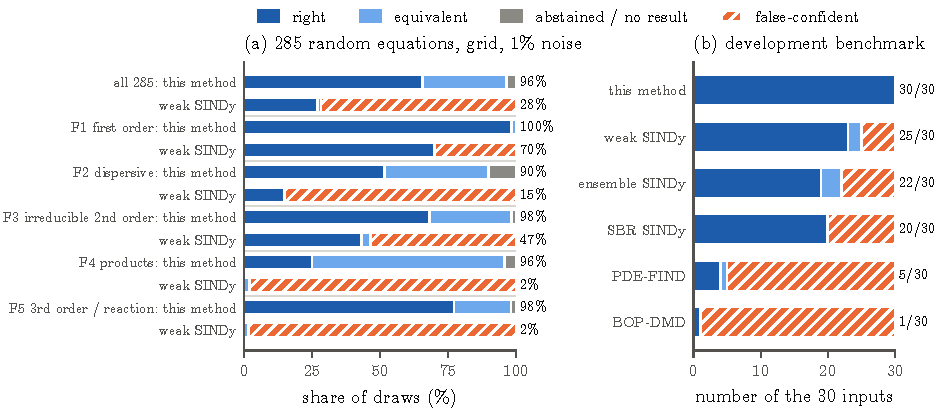
\includegraphics[width=\linewidth]{fig_evidence}
\caption{Outcomes. (a) Large benchmark, overall and per family: share of draws that are right, equivalent, abstained or
false-confident, with the right-or-equivalent share at the end of each bar. (b) Development benchmark: $10$ equations
$\times$ $3$ designs. Hatched: a wrong equation returned without any warning.}\label{fig:evidence}
\end{figure}

The method is right or equivalent on $275$ of $285$ draws ($96.5\%$) and false-confident on none; the exact one-sided
$95\%$ upper bound on its false-confident rate is $1.0\%$. Weak SINDy is right or equivalent on $81$ ($28.4\%$) and
false-confident on $204$. On the same draws the method succeeds where weak SINDy fails $194$ times and the reverse never
happens (exact sign test, $p=8\cdot10^{-59}$). The gap is largest exactly where the grouping principle predicts it:
on products of factors (F4) and on higher-order and reaction factors (F5) weak SINDy is right on one draw in fifty,
the method on $96$--$98\%$. Where both are right, the method's median relative coefficient error is $0.4\%$, against
$1.4\%$. Counting every one of the $15$ unfinished draws as a failure, the method is still right or equivalent on
$275/300=91.7\%$ (Wilson interval $88.0$--$94.3\%$); the unfinished draws are the slowest, not a random subset.

\paragraph{Development benchmark} Ten classical equations (transport, heat, advection--diffusion, Airy, Schr\"odinger,
beam, wave, Klein--Gordon, telegraph and the running example), each in three designs: a $64\times128$ grid with noise $1\%$,
the same grid with $5\%$, and $400$ scattered points with $5\%$. The defaults were tuned on these equations, so this is not
a held-out test; it compares the method with five baselines on classical cases (\cref{fig:evidence}(b),
\cref{tab:bench}). The method recovers all $30$ factor sets. The best baseline, weak SINDy, is right or equivalent on $25$
and false-confident on $5$, four of them products of factors. Repeating the two grid designs with three new fields and
noise draws each ($60$ independent inputs), the method is right on all $60$ with coefficient coverage $0.94$ at nominal
$0.90$; weak SINDy is false-confident on $13$.

\begin{table}[tbp]
\centering\small
\caption{Development benchmark: right or equivalent / false-confident, out of $10$ inputs per design, and the
repetition with independent fields and noise (out of $60$). Runtimes are wall-clock medians per input.}\label{tab:bench}
\begin{tabular}{@{}lcccccc@{}}
\toprule
Method & grid 1\% & grid 5\% & 400 pts 5\% & total & independent & median time\\
\midrule
this method        & 10 / 0 & 10 / 0 & 10 / 0 & 30 / 0 & 60 / 0 & 127 s\\
weak SINDy         & 10 / 0 & \phantom{1}7 / 3 & \phantom{1}8 / 2 & 25 / 5 & 47 / 13 & 3 s\\
ensemble SINDy     & \phantom{1}9 / 1 & \phantom{1}7 / 3 & \phantom{1}6 / 4 & 22 / 8 & -- & 5 s\\
SBR SINDy          & \phantom{1}8 / 2 & \phantom{1}6 / 4 & \phantom{1}6 / 4 & 20 / 10 & -- & 14 s\\
PDE-FIND           & \phantom{1}1 / 9 & \phantom{1}1 / 9 & \phantom{1}3 / 7 & \phantom{1}5 / 25 & -- & 0.6 s\\
BOP-DMD            & \phantom{1}1 / 9 & \phantom{1}0 / 10 & \phantom{1}0 / 10 & \phantom{1}1 / 29 & -- & 1.5 s\\
\bottomrule
\end{tabular}
\end{table}

\paragraph{Parameters and cost} The user-facing parameters are few: the starting and largest class ($C(3,4)$ and
$C(4,8)$), the detection threshold $z=3$, the goodness-of-fit level $10^{-3}$, the evidence margin of one nat, and the
number of posterior samples and bootstrap refits ($8$ and $16$); \SMalgo{} lists all of them. All were fixed during
development and left unchanged for the large benchmark. The price of exploring a whole class of factored structures on
every sample is time: a median of $127$\,s per input on the development benchmark and $13$ minutes on the random
equations, against seconds for library regression.

\begin{table}[b]
\centering\small
\caption{The kinds of claim made in the paper.}\label{tab:status}
\begin{tabularx}{\linewidth}{@{}>{\raggedright\arraybackslash}p{2.0cm}X@{}}
\toprule
Kind & Statements\\
\midrule
proved & groups are factors with overlap $\deltaP$ (\cref{thm:factor}); terms are not groups (\cref{prop:terms});
stability via $\gN$ (\cref{thm:hm}) and its Bayesian form (\cref{prop:bayes-angle}); identification and its limits on
finite data (\cref{thm:ident,prop:certify}); counting condition (\cref{prop:counting})\\
design rule & cluster modes onto curves, not terms onto a library; labels instead of ``identified''; decisions on the raw
observations; growth of the class instead of coefficient penalties; minimum-norm split of the overlap\\
measured & $275/285$ right or equivalent and $0$ confident wrong answers on random equations not used in development;
$30/30$ on the development benchmark and $60/60$ on its independent repetitions; coefficient coverage $0.94$ at nominal
$0.90$\\
\bottomrule
\end{tabularx}
\end{table}

\paragraph{What these numbers do and do not show} All inputs are synthetic and the noise is white; the large benchmark
uses one noise level, gridded data and one baseline. The claims we draw are therefore qualitative but sharp: on
equations whose symbol is a product of factors, or has factors of higher order, grouping by factors recovers the
structure where regression on a library of terms does not, and when the data do not suffice the labels and intervals
warn instead of returning a wrong equation.

\section{Discussion}\label{sec:discussion}
\paragraph{What is proved, what is designed, what is measured} \Cref{tab:status} separates the three kinds of claim. The
theorems hold under their hypotheses; the algorithm uses them as design rules, not as guarantees about its output; and
the numbers are evidence on synthetic data.

\paragraph{Limits that no amount of data removes} Some limits are theorems, and the output is built to show them rather
than hide them. \emph{Error floor}: in the Gaussian model of \cref{sec:group2} every unbiased estimator of the components
has variance at least $\noise^2/\gN$ in the worst direction, so closely aligned groups are intrinsically hard to separate.
\emph{No data-free threshold}: whether a numerical symbol ``factors'' depends on the noise level, which is why decisions are
made by evidence and not by a tolerance on coefficients. \emph{Repeated factors}: finite noisy data cannot distinguish
$P_i^2$ from two nearby factors, hence the label \UND. \emph{No certificate}: by \cref{prop:certify}, outputs are
compatibility statements with uncertainty, never identifications.

\paragraph{Beyond the linear ring} The two groupings do not depend on the equation being linear with constant
coefficients in one space dimension, and there are concrete reasons to expect the algorithm to extend. The matrix pencil
reads the temporal rates at every wavenumber vector $\kappa\in\R^d$ exactly as in one dimension, and the groups become
hypersurfaces $Q_j(\lambda,i\kappa)=0$ that grouping I can fit in the same way. For slowly varying coefficients a windowed
transform gives local rates $\lambda(\kappa;x_0)$, and each group becomes a family of curves indexed by position. For a
nonlinear equation, a short-time expansion shows that the flow is its linearization plus a quadratic interaction term,
so modes of the linearized flow can still be grouped on short windows. What does not carry over unchanged is the
theory: in higher dimension two factors can share a whole curve of zeros, the operators with variable coefficients form a
non-commutative algebra without unique factorization, and nonlinear solutions do not superpose. The first task in each
direction is therefore the one carried out here for the linear case: decide which pieces of the equation a solution
carries, how uniquely and how stably, and only then design the learning procedure around them (\SMbeyond).

\section{Conclusion}\label{sec:conclusion}
Groups are factors. This one statement, made precise by \cref{thm:factor} and its companions, determines what an
equation-learning algorithm should look for (modes on the curves of the factors), how it should combine evidence
(clustering factors across posterior samples), how it should measure uncertainty (through the Friedrichs angle), and
what it may claim (compatibility, never certification). On $285$ random equations never used in its development the
resulting method is right or equivalent on $96.5\%$ and never wrong without warning, while regression on a library of
terms is wrong without warning on most products and higher-order factors.

\section*{Code and data availability}
The code, the benchmark scripts and every stored result behind the numbers of this paper are at
\url{https://github.com/FlavioApric/pde-factor-fit}~\cite{Pri26code}; a snapshot is included in the supplementary
materials.


\Needspace{8\baselineskip}
\begin{thebibliography}{10}

\bibitem{BleJor06}
David~M. Blei and Michael~I. Jordan.
\newblock Variational inference for {D}irichlet process mixtures.
\newblock {\em Bayesian Analysis}, 1(1):121--143, 2006.

\bibitem{BruProKut16}
Steven~L. Brunton, Joshua~L. Proctor, and J.~Nathan Kutz.
\newblock Discovering governing equations from data by sparse identification of
  nonlinear dynamical systems.
\newblock {\em Proceedings of the National Academy of Sciences},
  113(15):3932--3937, 2016.

\bibitem{Deu01}
Frank Deutsch.
\newblock {\em Best Approximation in Inner Product Spaces}.
\newblock CMS Books in Mathematics. Springer, New York, 2001.

\bibitem{Ehr70}
Leon Ehrenpreis.
\newblock {\em Fourier Analysis in Several Complex Variables}.
\newblock Wiley-Interscience, New York, 1970.

\bibitem{FasKutBru22}
Urban Fasel, J.~Nathan Kutz, Bingni~W. Brunton, and Steven~L. Brunton.
\newblock Ensemble-{SINDy}: Robust sparse model discovery in the low-data,
  high-noise limit, with active learning and control.
\newblock {\em Proceedings of the Royal Society A}, 478(2260):20210904, 2022.

\bibitem{Gau62}
Walter Gautschi.
\newblock On inverses of {V}andermonde and confluent {V}andermonde matrices.
\newblock {\em Numerische Mathematik}, 4:117--123, 1962.

\bibitem{HirBarKut22}
Seth~M. Hirsh, David~A. Barajas-Solano, and J.~Nathan Kutz.
\newblock Sparsifying priors for {B}ayesian uncertainty quantification in model
  discovery.
\newblock {\em Royal Society Open Science}, 9(2):211823, 2022.

\bibitem{Hor90}
Lars H{\"o}rmander.
\newblock {\em An Introduction to Complex Analysis in Several Variables}.
\newblock North-Holland, Amsterdam, 3 edition, 1990.

\bibitem{HuaSar90}
Yingbo Hua and Tapan~K. Sarkar.
\newblock Matrix pencil method for estimating parameters of exponentially
  damped/undamped sinusoids in noise.
\newblock {\em IEEE Transactions on Acoustics, Speech, and Signal Processing},
  38(5):814--824, 1990.

\bibitem{Mal56}
Bernard Malgrange.
\newblock Existence et approximation des solutions des {\'e}quations aux
  d{\'e}riv{\'e}es partielles et des {\'e}quations de convolution.
\newblock {\em Annales de l'Institut Fourier}, 6:271--355, 1956.

\bibitem{MesBor21}
Daniel~A. Messenger and David~M. Bortz.
\newblock Weak {SINDy} for partial differential equations.
\newblock {\em Journal of Computational Physics}, 443:110525, 2021.

\bibitem{Obe90}
Ulrich Oberst.
\newblock Multidimensional constant linear systems.
\newblock {\em Acta Applicandae Mathematicae}, 20(1--2):1--175, 1990.

\bibitem{Pal70}
Victor~P. Palamodov.
\newblock {\em Linear Differential Operators with Constant Coefficients},
  volume 168 of {\em Grundlehren der mathematischen Wissenschaften}.
\newblock Springer, Berlin, 1970.

\bibitem{Pri26code}
Flavio Pricoco.
\newblock pde-factor-fit: reading the factor structure of linear {PDE}s from data.
\newblock \url{https://github.com/FlavioApric/pde-factor-fit}, 2026.
\newblock Software and benchmark data.

\bibitem{RaiPerKar17}
Maziar Raissi, Paris Perdikaris, and George~Em Karniadakis.
\newblock Machine learning of linear differential equations using {G}aussian
  processes.
\newblock {\em Journal of Computational Physics}, 348:683--693, 2017.

\bibitem{RudBruProKut17}
Samuel~H. Rudy, Steven~L. Brunton, Joshua~L. Proctor, and J.~Nathan Kutz.
\newblock Data-driven discovery of partial differential equations.
\newblock {\em Science Advances}, 3(4):e1602614, 2017.

\bibitem{SasKut22}
Diya Sashidhar and J.~Nathan Kutz.
\newblock Bagging, optimized dynamic mode decomposition for robust, stable
  forecasting with spatial and temporal uncertainty quantification.
\newblock {\em Philosophical Transactions of the Royal Society A},
  380(2229):20210199, 2022.

\bibitem{Sch10}
Peter~J. Schmid.
\newblock Dynamic mode decomposition of numerical and experimental data.
\newblock {\em Journal of Fluid Mechanics}, 656:5--28, 2010.

\end{thebibliography}

\end{document}
